\documentclass[12pt,a4paper,oneside]{book} %scrbook book report
\def\newblock{\hskip .11em plus .33em minus .07em}
\usepackage[english]{babel}
\usepackage{graphicx}
\graphicspath{figures/}
\usepackage{seecs}
\usepackage{url}
\usepackage{multirow}
\usepackage{amssymb,amsmath}
\usepackage{eucal}
\usepackage{nomencl}
\usepackage{natbib}
\usepackage{amsmath}
\usepackage[algoruled,vlined,linesnumbered,commentsnumbered,algochapter]{algorithm2e}
\usepackage{sfmath}

\setcounter{secnumdepth}{3}
\setcounter{tocdepth}{3}

\title{Automating Exchange of Educational Certificates Using DRESS}

\author{Umair Anwar}
\regno{2011-NUST-MS PhD-IT-049}
\degree{\MSIT}

\adviser{Dr. Sharifullah Khan}
\adviserAffiliation{NUST-SEECS}

\date{{June 2015}}

\setcounter{tocdepth}{2}
%\linespread{1.1}

\begin{document}
\maketitle

\evaluationcommitteeapproval{Dr. Hamid Mukhtar}{Dr. Sarah Shafiq Khan}{Mr. Mujtaba Haider}

\chapter*{Abstract}

 Student degree record is exchanged manually between educational institutes in Pakistan. In this paper, we put a push to recommend a data format and architecture for empowering these bodies to inter-exchange degree record digitally. To simplify its implementation, we recommend a mapping tool to semi-automatically create mappings between our standard and the institute data-sets.

%---------------------------------------------------------------------
\certificateoforiginality
%---------------------------------------------------------------------
\chapter*{Acknowledgment}
Up and above everything all glory to {\bfseries ALMIGHTY ALLAH}. The Beneficent, The most Merciful and Most Compassionate. It's a great blessing from Almighty Allah that gives me the health and strength to do this research work.\\

I would like to special thank the {\bfseries Supervisor}. \\

\begin{flushright} \textbf{Umair Anwar} \end{flushright}
%---------------------------------------------------------------------

\tableofcontents
%
%\printnomenclature{2.5cm}
%\nomenclature{DCF}{Distributed Coordination Function}
%
%
\chapter*{List of Abbreviations}

\begin{table}[h]
   % increase table row spacing, adjust to taste
    \renewcommand{\arraystretch}{1.3}
    \label{table:table1}
     \begin{tabular}{ll}
        \hline\hline
        % inserting double-line
            {\bfseries Abbreviations} & {\bfseries Descriptions} \\
            \hline                                      % inserts single-line
            DRES & Document Record Exchange Standard  \\
            DRESS & Document Record Exchange Standard Secured  \\
            SCHAC & Schema for Academia  \\
            LDAP & Lightweight Directory Access Protocol \\
            FVUSPEC & Finnish Virtual University Specifications  \\
            MLO & Meta-data for Learning Opportunities  \\
            WSDL & Web Service Description Language  \\
            EHEA & European Higher Education Area  \\
            ECTS & European Credit Transfer and Accumulation System  \\
            EA & Exchange Agreement  \\
            NQF & National Qualifications Framework  \\
            EQF & European Qualifications Framework  \\
            \hline                          % inserts single-line
    \end{tabular}
\end{table}

\listoffigures
\listoftables

%% \lstlistoflistings
%
\resetpagenumbering
%---------------------------------------------------------------------

\chapter{INTRODUCTION}\label{c-intro}
%-----------------------------------------------

The rest of the chapter is organized as follows. In Section 1.1, the problem statement is stated. In Section 1.2, thesis contributions are stated. In Section 1.3, we conclude the chapter with an outline for the rest of the thesis.

\section{Problem Statement}

Description of problem here...............

A formal problem statement is given as:

".................................."

\section{Thesis Contribution}

Our research work contributes in .................. areas.

All contributions of ................. are summarizing as follows:

\begin{itemize}
\item
Finding 1.
\item
Finding 2.
\end{itemize}

\section{Thesis Organization}

The rest of the thesis is organized as follows: \\

Chapter 2 discusses the state of the art related to the current research, and reviews the relevant literature aimed at finding .......................... \\

In Chapter 3, the .................... are discussed and then proposed methodology is presented. \\

In Chapter 4, the results are given along with detailed discussions. \\

In Chapter 5, the conclusion and future work is presented.

\chapter{LITERATURE REVIEW}\label{c-work}

There already exists a few standards and practices identified with exchanging degree or courses record. It is important to go through these, before proceeding onward to the new standard and the architecture we are proposing. We will review what these standards cover and what we can reuse.

\section{Bologna Process}

It intends to make European educational framework of standards engaging different countries in Europe to compare, contrast and make compatible their educational systems. \cite{bologna process}

To improve the mutual recognition of degrees and programs, education ministers from 29 countries signed bologna declaration in 1999. Other partaking countries joined the program later. \cite{improvement bologna process} Bologna process is quite often named as European Higher Education Area (EHEA). EHEA focuses on transferability and convergence adaption by 46 countries. This process benefits Europeans and it has its significance for other educational institutes and communities. a) The leading role of European institutes, b) the lessons that are learned in the implementation of the framework of standards, and c) the practices adopted guide the educational communities around the world. 2010 was marked as the deadline across Europe for implementing the agreed specifications. \cite{European Higher Education Area }

To meet the 2010 deadline, Spain started to implement the convergence of undergraduate engineering degrees that conformed EHEA in 2008. This standardization provided some opportunities for mobility and unified measurements. \cite{European Higher Education Area }




\section{Qualifications Exchange Standards}

    \subsection{European Qualifications Framework}
    EQF is an agreed reference framework that helps participating countries to compare national qualifications and make them more clear, readable and understandable across Europe. The point is to advance mobility of workers and learners. This was settled upon by European universities in 2008 to relate their national qualifications to EQF. The new qualifications from 2012 carry a reference to suitable EQF level.

    EQF comprises of eight reference levels, each showing what a learner knows and has the capacity to understand it. National qualifications of the partaking countries identify and relate with these eight levels raging from basic (level 1) to advanced (level 8). This simplifies qualification comparison in partaking countries supporting mobility of learners and empowering them to not repeat what they have already learned.
    
\begin{figure}[!t]
  \centering
  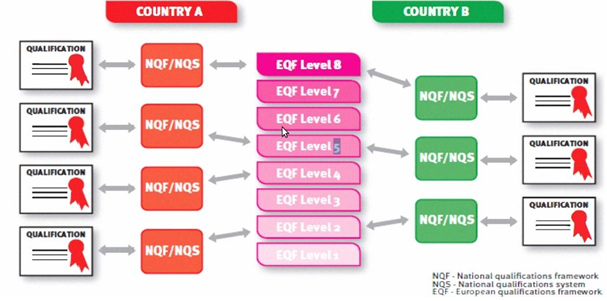
\includegraphics[width=9.25 in]{eqf.png}
  \caption{EQFs against NQFs}
  \label{fig:Fig1}
\end{figure}

    EQF concentrates on learning results as opposed to concentrating on learning inputs. It covers all types of education including professional, vocational and school education. It tries to validate formal and in addition informal education.

    \subsection{Europass}
    Collection of five documents which intend to ease mobility when seeking employment across Europe. These include the Curriculum Vitae, the Language Passport, the Mobility, the Diploma Supplement, and the Certificate Supplement. One can fill himself the Curriculum Vitae, and the Language Passport but the rest of the documents are issued by the related authorities. It follows a standard template format system, a layout. Same format helps to achieve neutrality and transparency while presenting one's skills.

    The motto as mentioned on the Europass website's homepage is as follows;
    "Five documents to make your skills and qualifications clearly and easily understood in Europe"

    Europass has defined XML schemas for CV and Language Passport. The documents can be exported in XML format when created on Europass. These exported XML documents can be imported to Europass and converted to HTML, PDF, Microsoft Word or ODT templates.

    Europass specifies JSON schema according to Internet Engineering Task Force's JSON specifications draft. The europass JSON vocabulary is close and similar to europass XML schema. The JSON objects for europass documents (CV and Language Passport) can be validated using Europass JSON validator.

    All these documents have some common XML schema attributes which describe document type, printed preferences.

    Europass does not explain details related to degrees or educational certificates in XML certificate.

        \subsubsection{Europass Curriculum Vitae}
        Europass Curriculum Vitae (ECV) is a template which one can create online and it can be exported in xml format. The ECV XML schema contains vocabularies related to document type, printing preferences, personal details, contact details, skills, and educational degrees and institutes. The XML vocabulary related to degree details is very little only to cover the scope of a CV.

        \subsubsection{Europass Language Passport}
        Europass Language Passport (ELP) is a template. One can create it online and export it in europass xml format. It contains XML vocabulary related to language skills and the scale of six values to score proficiency.

    \subsection{Schema for Academia}
    Schema for Academia (SCHAC) describes vocabulary related degrees and courses. The schema is written for LDAP (Lightweight Directory Access Protocol). It aims at promoting a common framework to inter-exchange data between educational institutes. It defines attributes that describe individuals and their LDAP profile

    \subsection{Dublin Core}
    The Dublin core is a simple meta-data standard consisting of set of elements to describe information resources on the network. There are two type of elements; simple and qualifiers. It has 15 simple elements and qualifiers which have additional three elements namely Audience, Provenance and RightsHolder. Qualifiers help in resource discovery.

\section{European Learner Mobility}
Some related work has been done recently and systems have been proposed based on the above mentioned standards. These are "The Mobility Project" and "The REST Mobility" projects.

    \subsection{The Mobility Project}
    It aimed to provide a platform and infrastructure for exchange of electronic data exchange between educational institutes. Infrastructure includes data format, architecture and the prototype software. The system will be called The Mobility later in this paper.

    The Mobility is peer to peer like architecture. Nodes exchange data using SOAP base web service. Other web services like XML-RPC and REST were not used due to their limitations. XML-RPC not have developer defined data-types and character set. REST does not imposes a standard specification, instead it follows set of rules and is used for speedy development of web service interface.

    The nodes represented the universities, and their number tends to change. So there was a need for system to maintain this record and UDDI was used. He did not recommend the central or delegated private registry instead gave advantages and disadvantages of both. Central single registry has all information at one place but also it a single point of failure.

    The software has two transport modules and each have web interface.

    Nagrozki proposed a new standard, defined its vocabulary re-using ideas taken from SCHAC to leverage ISO and RFC rules. Some like grade, credits were taken in inspiration from Eropass Mobility.

    Although The Mobility project was started by MUCI and CINECA, two European Higher Education Consortia. Many universities consortia, individual universities and companies joined in later on.

    \subsection{The REST Mobility}
    This is alternative implementation of The Mobility. Nagrozki's system used SOAP web service for data exchange. Karol created a RESTful implementation of the Mobility. The Mobility lacked data model. In The REST Mobility a data model is proposed since REST is resourceful. The model proposed not represents or intends to be a standard.

\section{Information Manifold}
Providing a uniform interface for querying data from many sources is the aim of Information Manifold. It enables a simple user to not worry about locating sources and manually combining results. This leads to concept of Deep Web. Data integration systems give users a common global schema called mediated schema for posting queries. To answer these queries semantic relationships called mappings are needed between mediated schema and the sources schema.

\section{MAPQFTOOL}
This tool helps comparing National Qualification Frameworks against European Qualifications Framework in Europe. This automates the process of creating mappings between these frameworks and stores the mappings in the database.

Related to the \cite{umair} research related to the regression models for predictions is concerned, Ali et al.~\cite{ali} discussed the application of linear regression for future prediction using {\it SPSS} (Statistical Package for the Social Sciences). They found the P-values, beta scores, $R^2$, mean and standard deviation parameters that helped to learn good models for future prediction.

These regressions were found using response variable $y$ and predictor variable $x$ as shown in equations~\ref{eq2.13}-\ref{eq2.16}.
%
\begin{equation}
  y  =  w_0 + w_1 * x \; \mbox{(Linear)}
  \label{eq2.13}
\end{equation}
%
\begin{equation}
  y = w_0 + w_1 * x + w_2 * x^2 \; \mbox{(Quadratic)}
  \label{eq2.14}
\end{equation}
%
\begin{equation}
  y = w_0 + w_1 * x + w_2 * x^2 + w_3 * x^3 \; \mbox{(Cubic)}
  \label{eq2.15}
\end{equation}
%
\begin{equation}
  y = w_0 * x^{w_1} \; \mbox{(Power)}
  \label{eq2.16}
\end{equation}
%
\noindent where $w_0$, $w_1$, $w_2$,and $w_3$ are regression coefficients.

\chapter{REQUIREMENTS ANALYSIS}\label{c-requirements-analysis}
For two universities to exchange data, they have to create an agreement first. The agreement will have the list of documents for which data exchange is available and exchange secrets will be generated.

\chapter{Architecture and Design}\label{c-architecture-design}
From use cases and the business requirements, we suggest student exchange system will have distributed architecture. Each university has its own data and signs agreements independently for exchanging data with other universities. Each can be a requester plus a provider of data. The circles/nodes in the figure below represent universities. The arrows represent exchange of data.
This peer to peer like distribute architecture has benefits over adding a middle agent or central server in the system.
1.	Avoidance from single point of failure.
2.	Lesser load.
3.	Each university having control over its own data and thus building trust in the system.

There are some choices to be made at this point. We will be using web services for exchanging data as they provide a high abstraction from network issues and use well known standards like XML over HTTP. There are some XML based data exchange protocols on web. These are XML-RPC, SOAP, and REST.

The nodes will exchange data using SOAP based web service in our system.  We chose SOAP as it forces to follow a formal standard and supports developer defined data types.

The number of universities can increase when agreements are signed with new universities for exchange data. The web service URLs need to be saved so that requester can retrieve this URL and request that university. This can be achieved by developing a custom system or using UDDI. UDDI is a standard used to discover and save web services URLs. Now we have to make a choice. UDDI can be global or each requesting node can have its own private UDDI registry. We will use private registry to avoid single point of failure and to minimize load.


\chapter{IMPLEMENTATION}\label{c-implement}
In this chapter, the methodology that is used for modeling is explained.

Methodology Here .............................

\chapter{RESULTS AND DISCUSSION}\label{c-results}

This chapter presents detailed results along with relevant discussions. In this chapter, Section 4.1 explains the .................... results with detailed discussions; while Section 4.2 explains the ........... results with detailed discussions.

\section{Section Heading Here}

This section presents the results of ................

\subsection{Sub-Section Heading Here}

In order to perform ................

we have found that the pH is high in June and November as shown in Fig.~\ref{fig:Fig4}.  Fig.~\ref{fig:Fig4} shows........ Moreover, the trends for the remaining parameters are briefly described in Table~\ref{table:table13}.

\begin{figure}[!t]
  \centering
  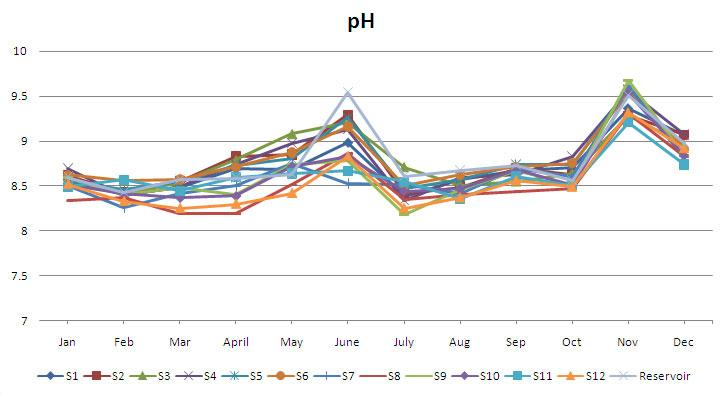
\includegraphics[width=3.25 in]{Fig-1.jpg}
  \caption{Month-wise pH Trend of Streams}
  \label{fig:Fig4}
\end{figure}


\begin{table}[!t]
  \begin{center}\scriptsize
     % increase table row spacing, adjust to taste
      \renewcommand{\arraystretch}{1.3}
      \caption{Month-wise Parametric Trend}
      \label{table:table13}
      \begin{tabular}{ll}
          \hline\hline
          % inserting double-line
              {\bfseries Parameter} & {\bfseries Trend} \\
              \hline                                      % inserts single-line
              Alkalinity & High values in February as compared to other months\\
              \hline                          % inserts single-line
      \end{tabular}
  \end{center}
\end{table}

\chapter{CONCLUSION AND FUTURE WORK}\label{c-conclusion}

In this chapter, the conclusion with a summary of the research findings along with future directions is presented.

\section{Conclusion}
Conclusion Here.........

\section{Future Work}
In future, the ..............

\begin{thebibliography}{10}

\bibitem{umair}
M. Ali, H. Qureshi, and M. S. Akhtar (2013), \emph{Analysis of growth in Students Intake and Degree Awarding Contribution: A Comparison of Stanford and MIT}, MLDM 2013: International Conference on Machine Learning and Data Mining, in press.

\bibitem{bologna process}
http://www.ehea.info/Uploads/Irina/Bologna%20beyond%202010.pdf

\bibitem{MAPQFTOOL}
P. Pouyioutas, H. Gjermundrod, and M. Michael, "MAPQFTOOL: A software tool to support national qualifications frameworks," Information Society (i-Society), 2011 International Conference on, pp. 198-203, Jun. 2011.

\bibitem{The Mobility Project}
Rafal Nagrodzki, "The Mobility Project," Institue of Informatics, University of Warsaw, Warsaw, Master's Thesis 2009.

\bibitem{European Higher Education Area }
A. Duran, Y.B. Moon, and E. Giraldo, "Work in progress - the European Higher Education Area ("Bologna process") in Engineering Education in Spain," Frontiers in Education Conference, 2009. FIE '09. 39th IEEE, pp. 1,2, Oct. 2009.

\bibitem{Integration of Services in the Mobility Project}
Karol Kanski, "Integration of Services in the Mobility Project," Institute of Informatics, University of Warsaw, Warsaw, Master's Thesis 2011.

\bibitem{Data integration: the teenage years}
Alon Halevy, Anand Rajaraman, and Joann Ordille, "Data integration: the teenage years," In Proceedings of the 32nd international conference on Very large data bases (VLDB '06), pp. 9-16, 2006.

\bibitem{improvement bologna process}
Szentirmai, L.; Radacs, L., "Improvement of academic and research standards of higher engineering education in light of Bologna process," Emerging eLearning Technologies \& Applications (ICETA), 2012 IEEE 10th International Conference on , vol., no., pp.381,386, 8-9 Nov. 2012

\end{thebibliography}

\end{document} 